\documentclass[conference]{IEEEtran}
\IEEEoverridecommandlockouts

\usepackage{cite}
\usepackage{amsmath,amssymb,amsfonts}
\usepackage{graphicx}
\usepackage{textcomp}
\usepackage{xcolor}
\usepackage{booktabs}
\usepackage{url}
\usepackage{hyperref}
\hypersetup{colorlinks=true, linkcolor=blue, citecolor=blue, urlcolor=blue}

% Suppress underfull hbox warnings from tight IEEE two-column layout
\setlength{\emergencystretch}{5em}
\tolerance=2000

\def\BibTeX{{\rm B\kern-.05em{\sc i\kern-.025em b}\kern-.08em
    T\kern-.1667em\lower.7ex\hbox{E}\kern-.125emX}}

\begin{document}

\title{Turkey Logistics Decision-Support System:\\
A Transportation-Problem Platform with Disruption Simulation,\\
Demand Forecasting, Facility Location, and Multi-Period Planning}

\author{
  \IEEEauthorblockN{Fatih Bahad\i r Karaku\c{s}}
  \IEEEauthorblockA{
    \textit{Email: bahadirkarakus261@gmail.com}
  }
}

\maketitle

%-----------------------------------------------------------------------
\begin{abstract}
This paper presents a web-based Decision-Support System (DSS)
for optimising freight distribution across a Turkey-wide logistics network
composed of five production centres and eight regional warehouses.
The system formulates the distribution problem as a linear programming (LP)
transportation model and solves it with the CBC simplex solver via PuLP.
Beyond deterministic optimisation, the platform integrates eight analytical
modules: sensitivity analysis via dual variables and reduced costs;
Monte Carlo simulation of demand uncertainty; a multi-objective Pareto
frontier balancing cost against travel time; a scenario manager for
rapid what-if comparisons; a four-quarter multi-period LP with inventory
carryover; Holt double-exponential demand forecasting; supply disruption
simulation with route re-optimisation; and a p-median binary MIP for
facility location.
A Streamlit web dashboard with eleven interactive tabs delivers maps
(Folium), Sankey diagrams, heatmaps, and downloadable PDF/Excel reports,
while a FastAPI backend exposes all analytical endpoints as a REST API.
Results demonstrate that routing 1{,}610 units across 8--10 active routes
achieves minimum total transport costs of approximately
\textlira 118{,}000--168{,}000 depending on the operating scenario,
with shadow-price analysis identifying Antalya and Gaziantep as the
binding demand constraints most sensitive to cost changes.
\end{abstract}

\begin{IEEEkeywords}
transportation problem, linear programming, p-median facility location,
demand forecasting, disruption simulation, Streamlit, logistics optimisation
\end{IEEEkeywords}

%=======================================================================
\section{Introduction}
\label{sec:intro}

Efficient freight distribution is a critical challenge for manufacturers
operating national supply chains.
Turkey's geography---spanning Thrace, the Aegean, central Anatolia, the
Black Sea coast, and the Mediterranean---creates substantial variation in
transport distances, road tolls, and seasonal demand patterns.
Practitioners often resort to manual allocation or heuristic spreadsheet
tools that cannot guarantee optimality or quantify the cost of uncertainty.

This work describes a Decision-Support System (DSS) that addresses these
shortcomings by embedding a classical LP transportation model inside an
interactive web application with eight analytical extensions.
The platform allows analysts to:
\begin{itemize}
  \item select predefined scenarios or customise supply and demand in real time;
  \item impose a CO\textsubscript{2} emission budget as a hard LP constraint;
  \item run sensitivity analysis to identify binding constraints;
  \item simulate cost distributions under stochastic demand (Monte Carlo);
  \item trace the Pareto frontier between cost and travel-time;
  \item plan over four quarters with inventory carryover (multi-period LP);
  \item forecast future demand with Holt exponential smoothing;
  \item simulate supply disruptions and inspect automatic re-routing;
  \item find optimal hub locations with a p-median binary MIP.
\end{itemize}

The remainder of this paper is organised as follows.
Section~\ref{sec:problem} states the mathematical formulation.
Section~\ref{sec:cost} describes the cost estimation model.
Section~\ref{sec:solution} outlines the solution approach.
Section~\ref{sec:architecture} summarises the system architecture.
Section~\ref{sec:results} presents deterministic optimisation results.
Sections~\ref{sec:scenario}--\ref{sec:pareto} cover the core analytics.
Section~\ref{sec:extensions} describes the four extensions.
Section~\ref{sec:conclusion} concludes.

%=======================================================================
\section{Problem Formulation}
\label{sec:problem}

\subsection{Network Structure}

The logistics network consists of production centres
$I = \{$\.Istanbul, Ankara, \.Izmir, Bursa, Adana$\}$ and
warehouses
$J = \{$Konya, Kayseri, Trabzon, Gaziantep, Antalya,
Samsun, Eski\c{s}ehir, Diyarbak\i r$\}$.
Each source $i \in I$ has supply capacity $s_i$ (units)
and each warehouse $j \in J$ has demand $d_j$ (units).
The network is \emph{unbalanced}: total supply exceeds total demand
($\sum_i s_i = 2{,}650 > \sum_j d_j = 1{,}610$ units).

\subsection{Decision Variables}

$$x_{ij} \geq 0 \quad \forall\, i \in I,\; j \in J$$

\subsection{Objective Function}

\begin{equation}
  Z = \sum_{i \in I}\sum_{j \in J} c_{ij}\, x_{ij}
  \label{eq:objective}
\end{equation}

\subsection{Constraints}

\begin{align}
  \sum_{j \in J} x_{ij} &\leq s_i \quad \forall\, i \in I
  \label{eq:supply} \\
  \sum_{i \in I} x_{ij} &\geq d_j \quad \forall\, j \in J
  \label{eq:demand} \\
  \sum_{i,j} e_{ij}\, x_{ij} &\leq B
  \label{eq:co2}
\end{align}

where $e_{ij}$ (kg CO\textsubscript{2}/unit) is the per-unit emission factor
derived from IPCC diesel combustion coefficients \cite{ipcc},
and $B$ is an optional emission budget (constraint omitted when not active).
The model has $|I| \cdot |J| = 40$ decision variables and up to
$|I| + |J| + 1 = 14$ functional constraints.

%=======================================================================
\section{Cost Estimation Model}
\label{sec:cost}

Unit transport cost $c_{ij}$ is derived from a per-trip cost model:

\begin{equation}
  c_{ij} = \frac{
    d_{ij}\!\cdot\!\frac{L}{100}\!\cdot\! p_f
    \;+\; \frac{d_{ij}}{v}\!\cdot\! w
    \;+\; \tau_{ij}
    \;+\; f
  }{q}
  \label{eq:cost}
\end{equation}

Parameters: road distance $d_{ij}$ (km); fuel consumption
$L/100 = 30$ L/100 km; diesel price $p_f = 40$ TL/L;
average speed $v = 80$ km/h; driver wage $w = 150$ TL/h;
route toll $\tau_{ij}$ (TL); fixed fee $f = 200$ TL;
truck capacity $q = 25$ units.
A fuel multiplier $\mu_f$ scales the cost matrix for fuel price shocks.
CO\textsubscript{2} emissions per unit are computed as
$e_{ij} = d_{ij} \cdot \frac{L}{100} \cdot 2.68 / q$
using an IPCC diesel emission factor of 2.68 kg CO\textsubscript{2}/L.

%=======================================================================
\section{Solution Approach}
\label{sec:solution}

The model is implemented with PuLP \cite{pulp} and the CBC simplex
solver \cite{cbc} (output suppressed).
For a transportation LP of this size (40 variables, 13--14 constraints),
the simplex method converges in under 50 pivots in milliseconds.
Post-solve, the system extracts shipment plan, slack, demand fulfilment,
and dual variables for downstream analytics.

%=======================================================================
\section{System Architecture}
\label{sec:architecture}

\begin{figure}[htbp]
  \centering
  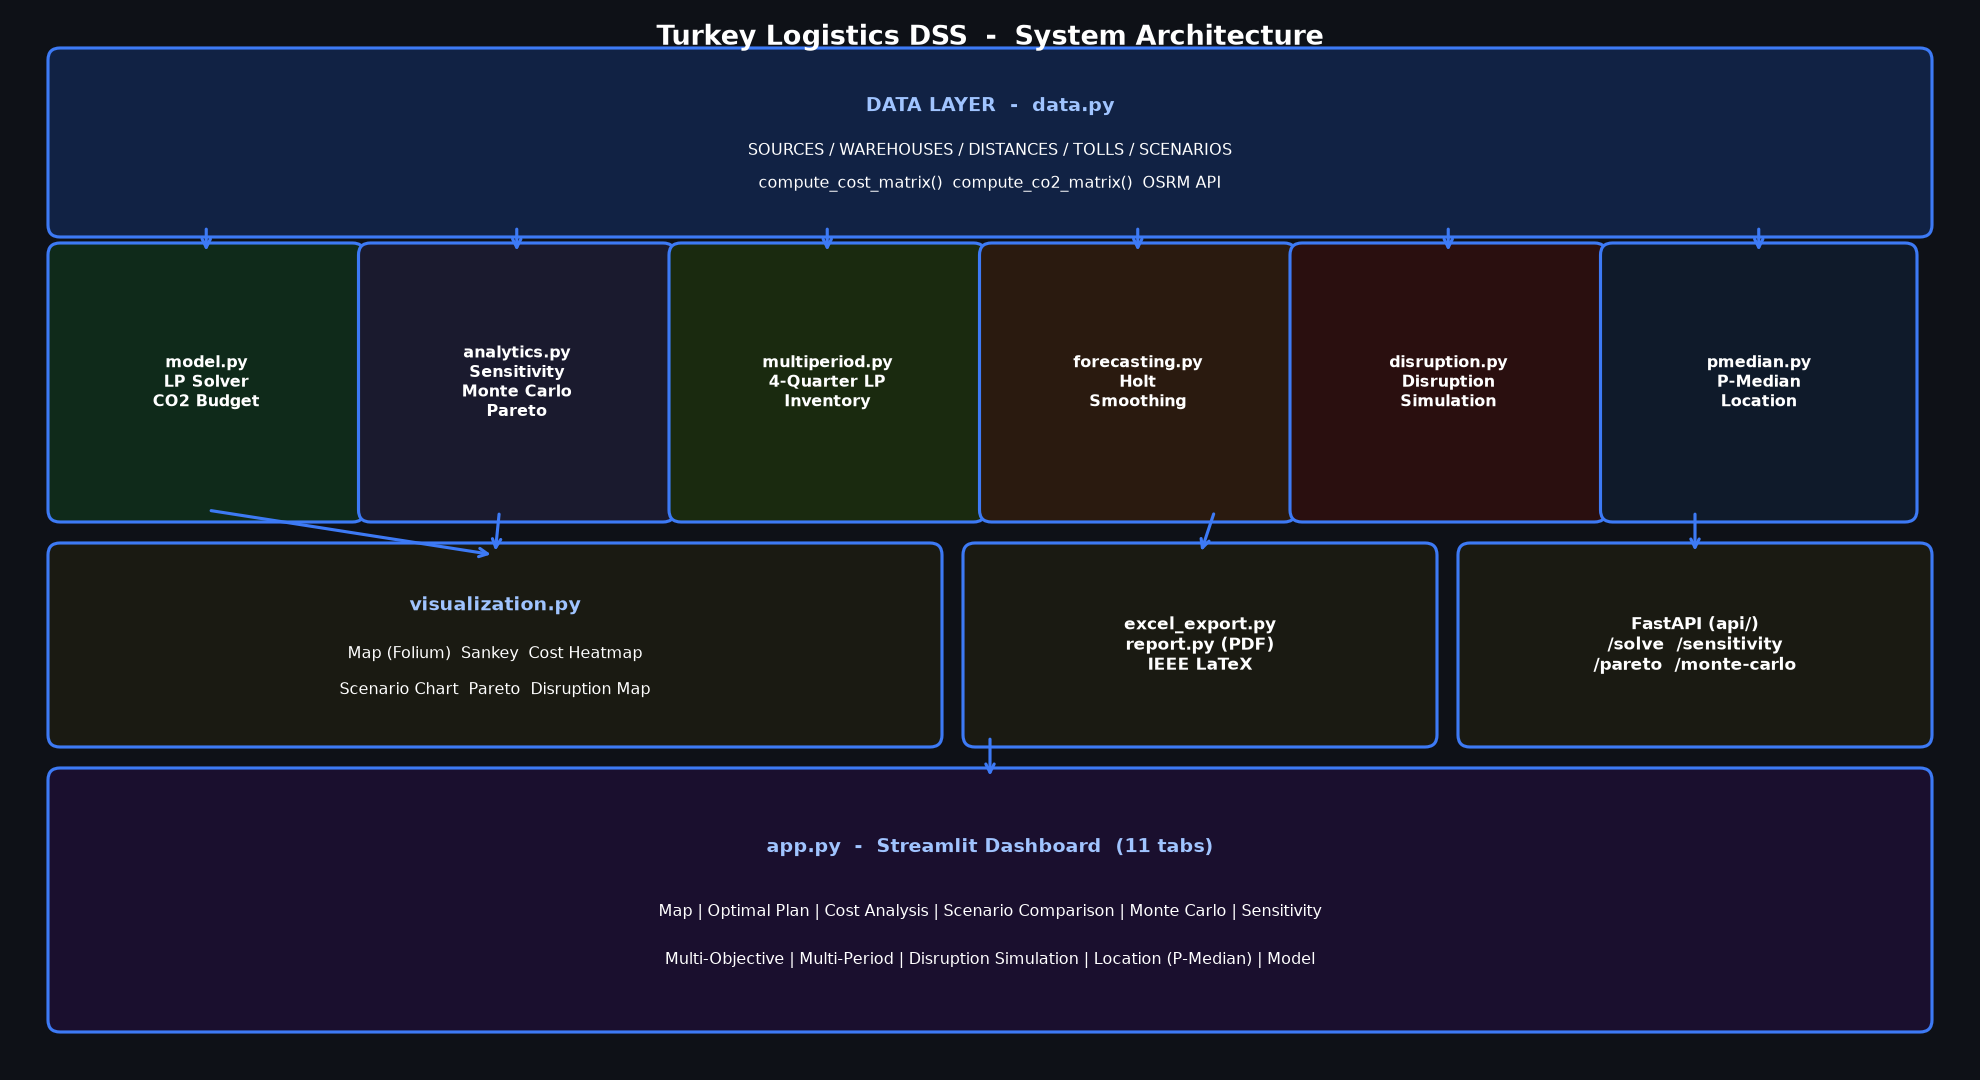
\includegraphics[width=\linewidth]{fig_architecture.png}
  \caption{System architecture: data layer, six solver/analytics modules,
           visualisation, FastAPI, and the eleven-tab Streamlit front-end.}
  \label{fig:architecture}
\end{figure}

The DSS is structured as nine Python modules (Fig.~\ref{fig:architecture}).
\textbf{data.py} holds the network topology, scenario definitions, CO\textsubscript{2}
parameters, and the OSRM API client.
\textbf{model.py} wraps the PuLP LP (with optional CO\textsubscript{2} cap).
\textbf{analytics.py} implements sensitivity analysis, Monte Carlo simulation,
and Pareto enumeration.
\textbf{multiperiod.py} formulates the four-quarter LP with inventory balance.
\textbf{forecasting.py} provides Holt double-exponential smoothing.
\textbf{disruption.py} compares base and disrupted optimal plans.
\textbf{pmedian.py} solves the p-median binary MIP.
\textbf{visualization.py} builds all Plotly and Folium figures.
\textbf{app.py} is the Streamlit entry point (eleven-tab dashboard).
A \textbf{FastAPI} backend (\texttt{api/}) exposes \texttt{/solve},
\texttt{/sensitivity}, \texttt{/monte-carlo}, and \texttt{/pareto} as a
REST API; a Docker Compose file wires the two services together.

\begin{figure}[htbp]
  \centering
  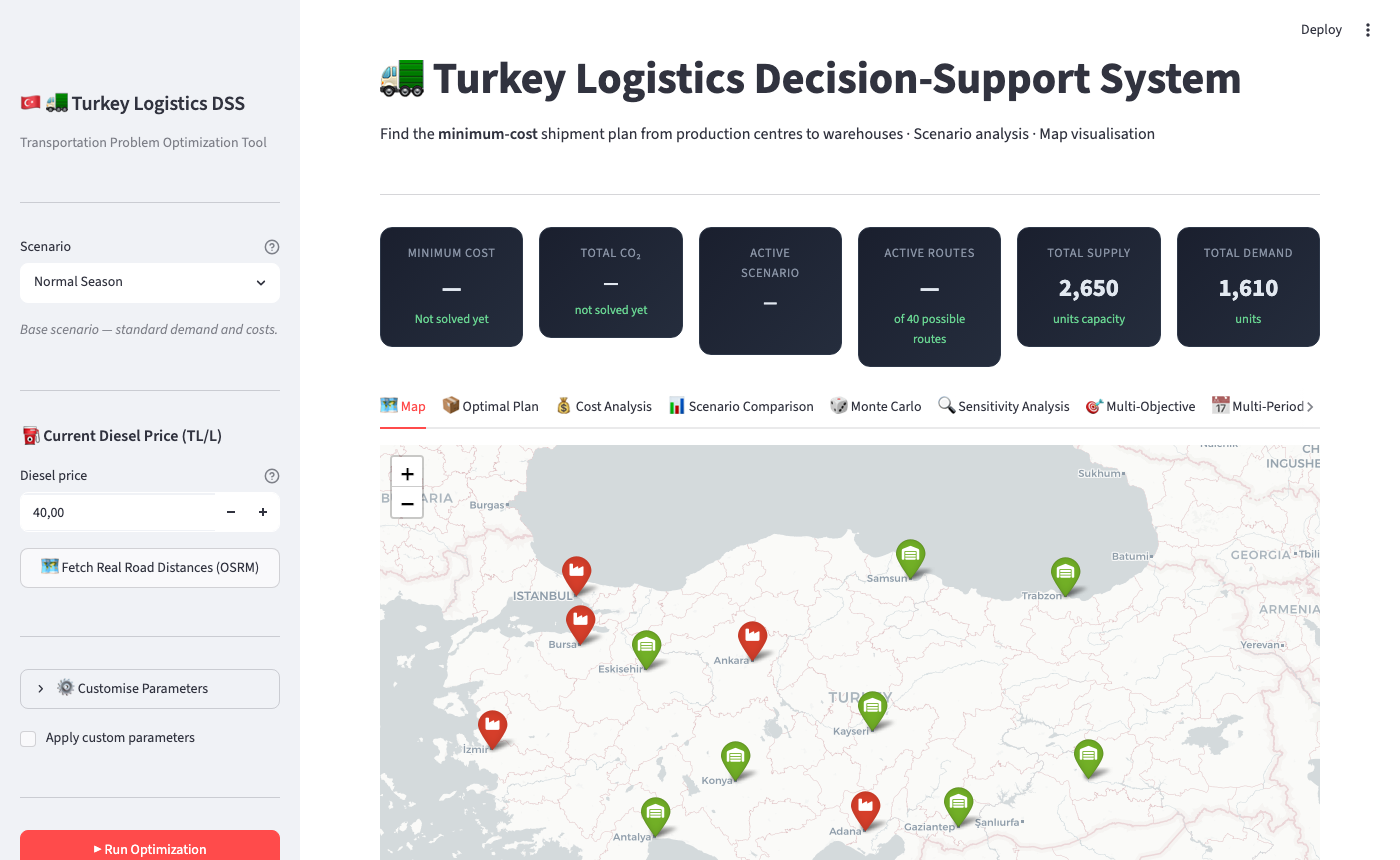
\includegraphics[width=\linewidth]{fig_interface.png}
  \caption{Main dashboard: KPI cards and the eleven-tab interface.}
  \label{fig:interface}
\end{figure}

%=======================================================================
\section{Optimisation Results}
\label{sec:results}

\begin{table}[htbp]
\caption{Production Centre Capacities}
\label{tab:supply}
\centering
\begin{tabular}{lc}
\toprule
Production Centre & Capacity (units) \\
\midrule
\.Istanbul & 800 \\
Ankara     & 600 \\
\.Izmir    & 500 \\
Bursa      & 400 \\
Adana      & 350 \\
\midrule
\textbf{Total} & \textbf{2{,}650} \\
\bottomrule
\end{tabular}
\end{table}

\begin{table}[htbp]
\caption{Warehouse Demands (Normal Season)}
\label{tab:demand}
\centering
\begin{tabular}{lc}
\toprule
Warehouse    & Demand (units) \\
\midrule
Konya        & 250 \\
Kayseri      & 200 \\
Trabzon      & 150 \\
Gaziantep    & 220 \\
Antalya      & 280 \\
Samsun       & 180 \\
Eski\c{s}ehir & 160 \\
Diyarbak\i r & 170 \\
\midrule
\textbf{Total} & \textbf{1{,}610} \\
\bottomrule
\end{tabular}
\end{table}

Under the Normal Season scenario, the CBC solver finds the optimal
solution in under 10\,ms with a total cost of approximately
\textlira 118{,}000.
Eight to ten routes carry positive flow; the remaining slack of
1{,}040 units resides primarily at \.Istanbul and \.Izmir.

\begin{figure}[htbp]
  \centering
  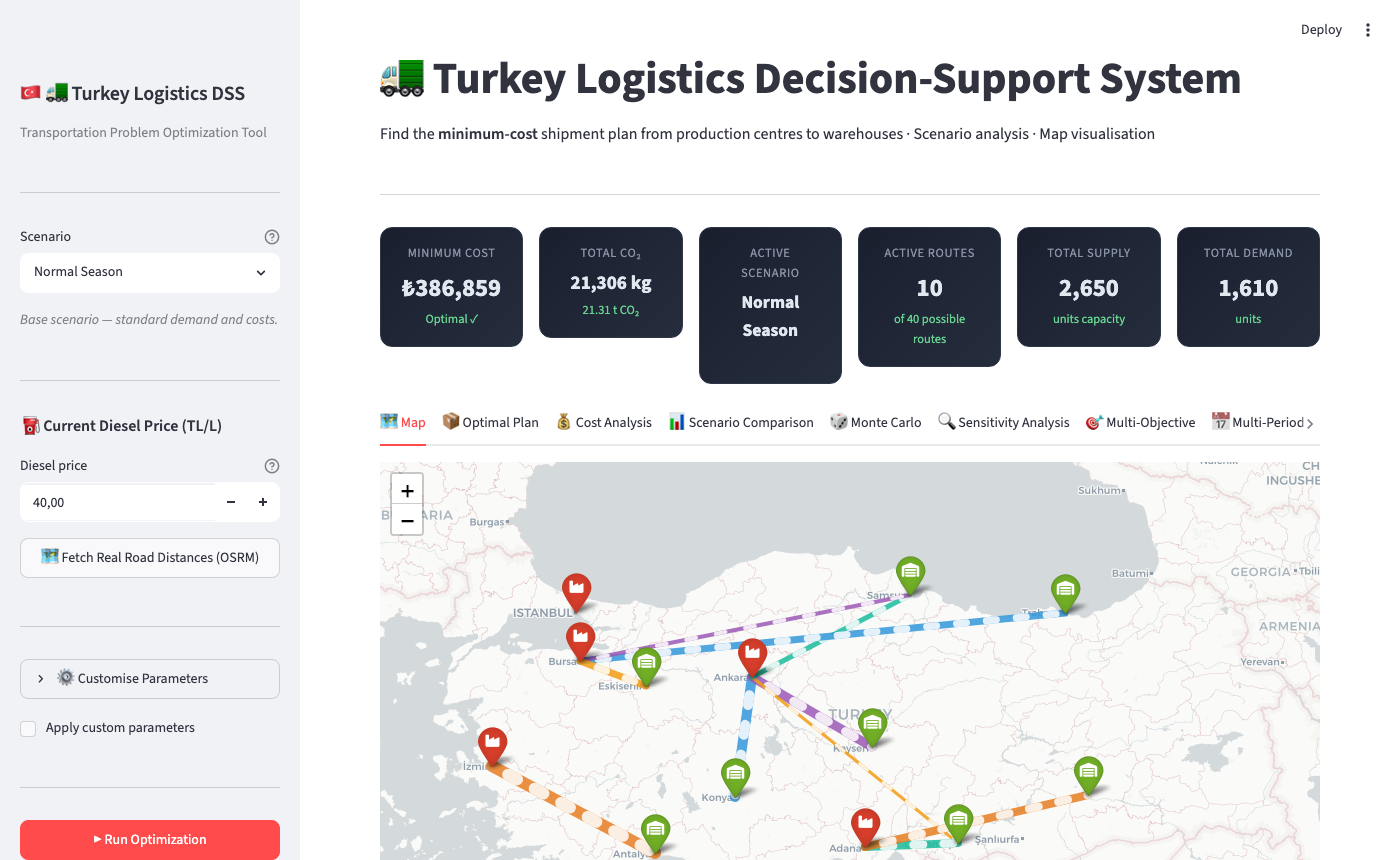
\includegraphics[width=\linewidth]{fig_map.png}
  \caption{Optimal shipment routes on the interactive Folium map.
           Line thickness is proportional to shipment volume.}
  \label{fig:map}
\end{figure}

\begin{figure}[htbp]
  \centering
  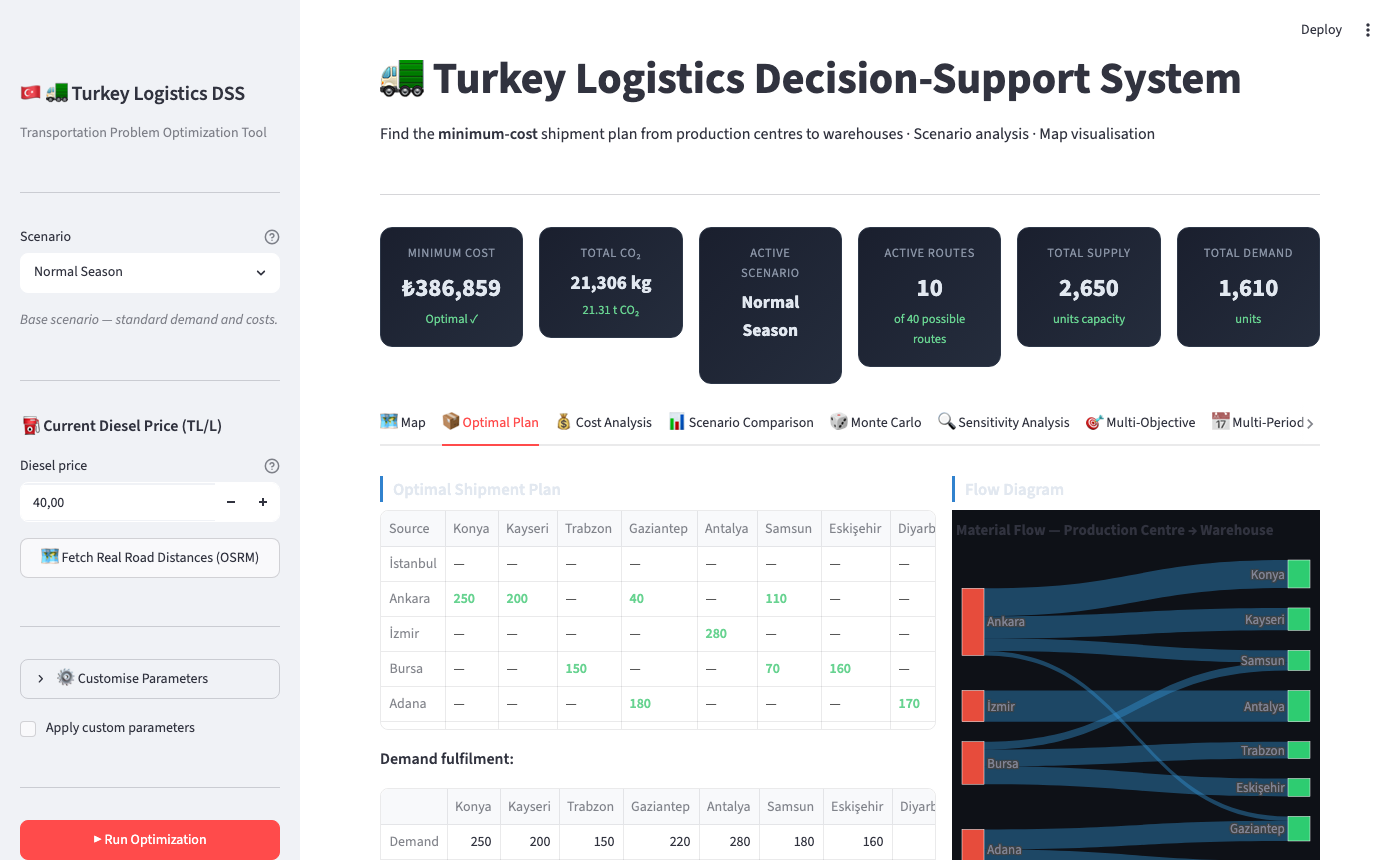
\includegraphics[width=\linewidth]{fig_sankey.png}
  \caption{Sankey flow diagram: unit volumes from each production centre
           to each served warehouse.}
  \label{fig:sankey}
\end{figure}

\begin{figure}[htbp]
  \centering
  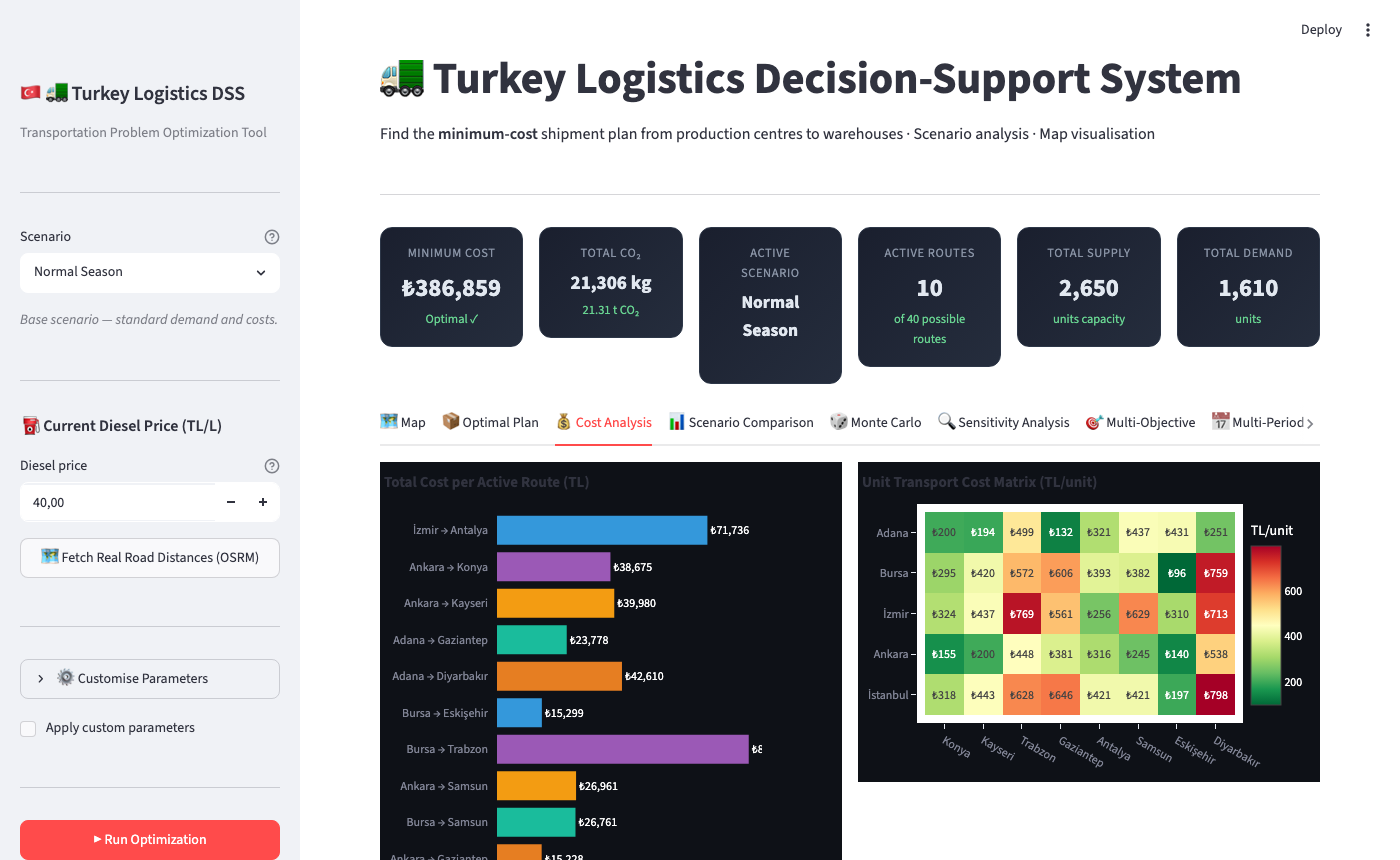
\includegraphics[width=\linewidth]{fig_cost.png}
  \caption{Cost breakdown per active route (TL), sorted by total cost.}
  \label{fig:cost}
\end{figure}

%=======================================================================
\section{Scenario Analysis}
\label{sec:scenario}

Four predefined scenarios capture common operating conditions:
\textbf{Normal Season} (base, $\mu_f = 1.0$),
\textbf{Summer Season} (Antalya $+40\%$, Trabzon $+20\%$, Samsun $+15\%$),
\textbf{Fuel Increase} ($\mu_f = 1.20$, demand unchanged), and
\textbf{Winter Season} (inland cities $+10$--$20\%$,
coastal resorts $-20$--$30\%$, $\mu_f = 1.05$).

\begin{figure}[htbp]
  \centering
  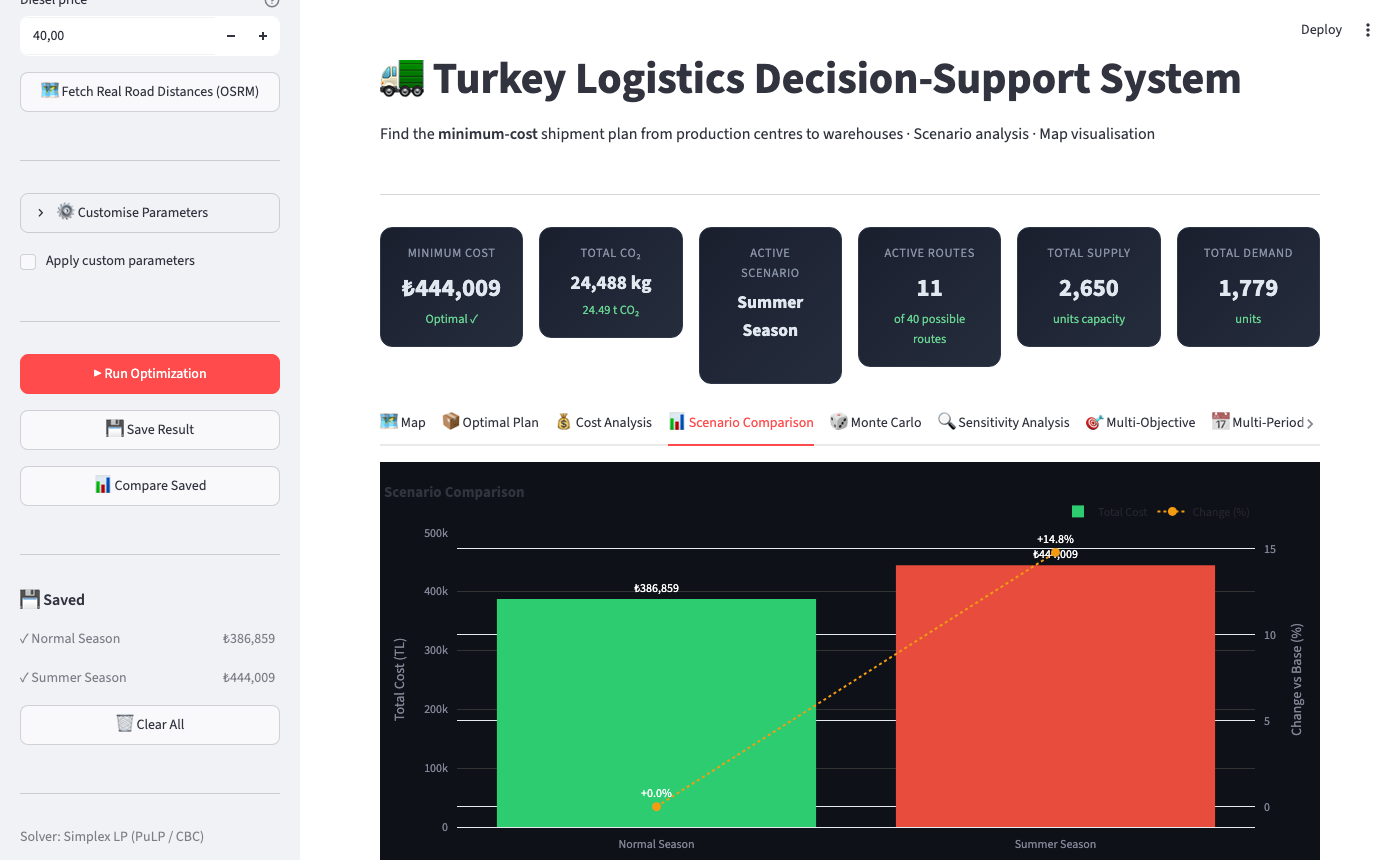
\includegraphics[width=\linewidth]{fig_scenario.png}
  \caption{Scenario comparison: total cost and percentage deviation
           from the Normal Season baseline.}
  \label{fig:scenario}
\end{figure}

%=======================================================================
\section{Sensitivity Analysis}
\label{sec:sensitivity}

Dual variables are extracted via \texttt{constraint.pi} (shadow prices)
and \texttt{variable.dj} (reduced costs) after solving.
The shadow price of a supply constraint equals the cost reduction achievable
by relaxing capacity by one unit; the shadow price of a demand constraint
equals the cost increase required to serve one additional unit.

\begin{figure}[htbp]
  \centering
  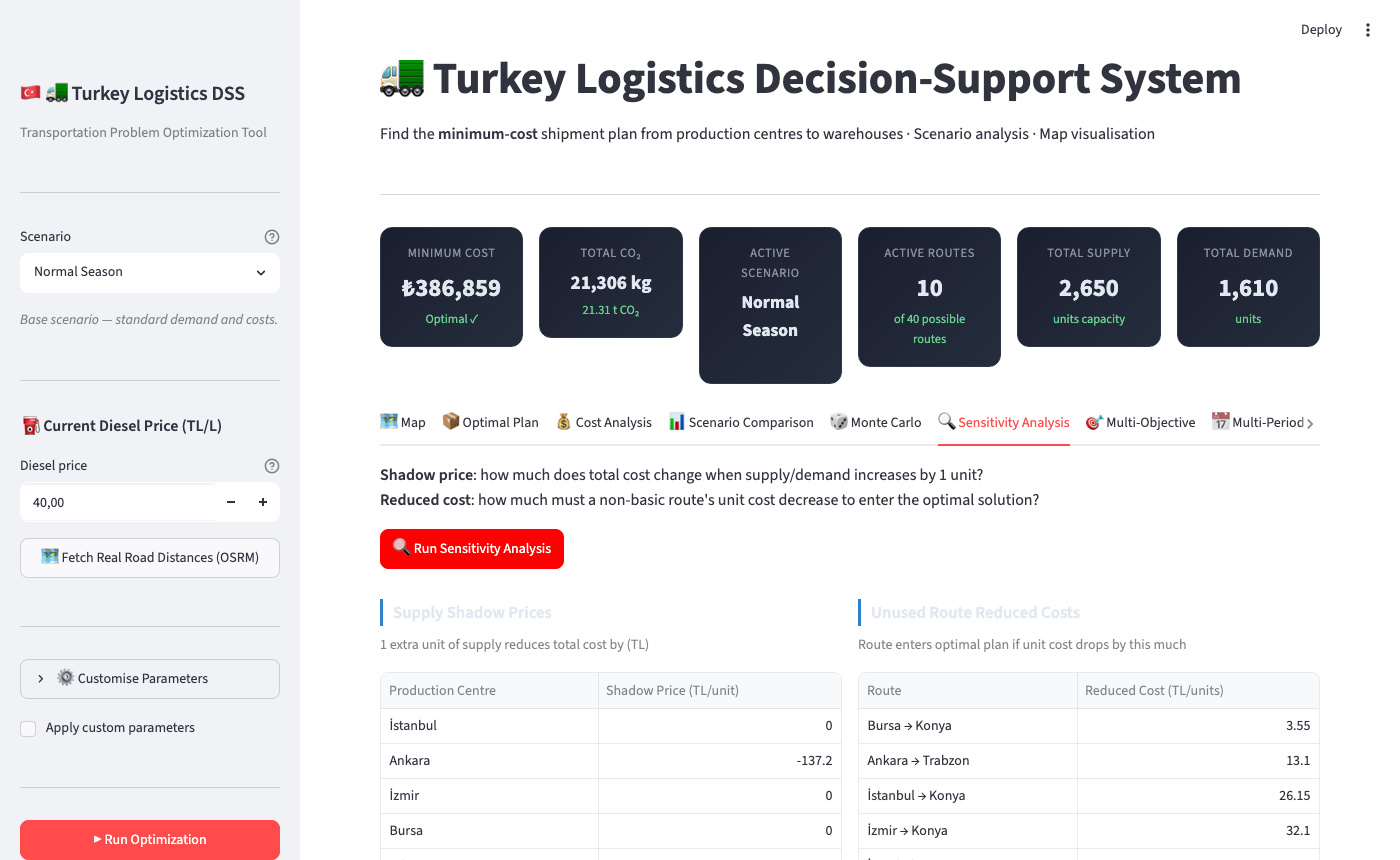
\includegraphics[width=\linewidth]{fig_sensitivity.png}
  \caption{Shadow prices for supply and demand nodes; reduced costs for
           inactive routes.}
  \label{fig:sensitivity}
\end{figure}

In the base case, Antalya and Gaziantep show the highest demand shadow
prices; \.Istanbul has a near-zero supply shadow price, confirming its
large idle capacity is non-binding.

%=======================================================================
\section{Monte Carlo Simulation}
\label{sec:montecarlo}

Warehouse demand is modelled as a truncated normal:
$\tilde{d}_j \sim \mathcal{TN}(d_j,\;(\text{CV}\cdot d_j)^2)$
with default $N = 300$ iterations and $\text{CV} = 0.15$.

\begin{figure}[htbp]
  \centering
  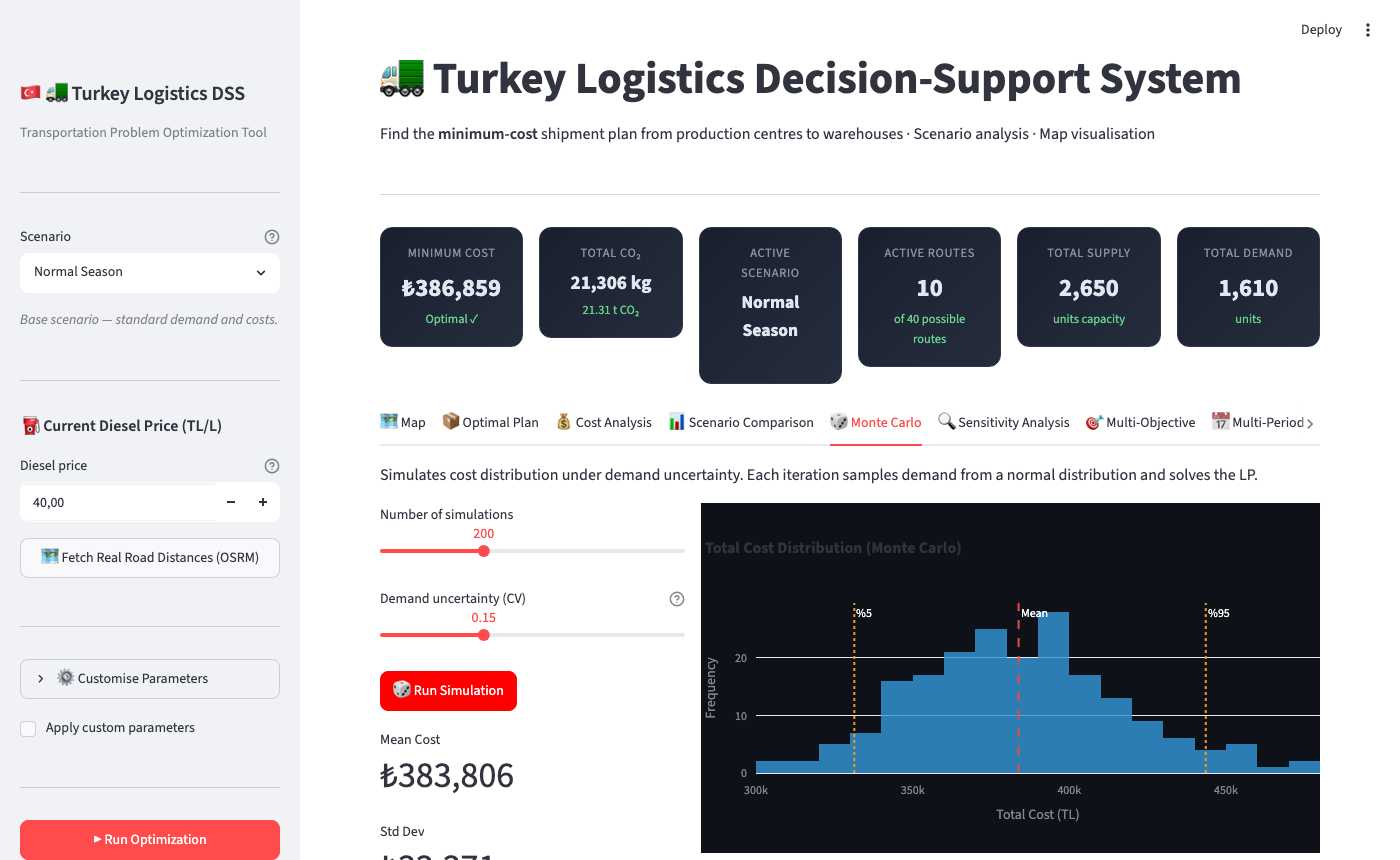
\includegraphics[width=\linewidth]{fig_montecarlo.png}
  \caption{Monte Carlo cost histogram (300 iterations, CV = 0.15)
           and route reliability heatmap.}
  \label{fig:montecarlo}
\end{figure}

The 90\% cost interval spans $\pm 8$--$12\%$ around the deterministic
optimum; core routes maintain $>95\%$ reliability.

%=======================================================================
\section{Multi-Objective Pareto Frontier}
\label{sec:pareto}

Weighted-sum scalarisation ($\alpha \in [0,1]$) solves:
$\min\;\alpha\,\hat{Z}_\text{cost} + (1-\alpha)\,\hat{Z}_\text{time}$
tracing non-dominated cost--time pairs.

\begin{figure}[htbp]
  \centering
  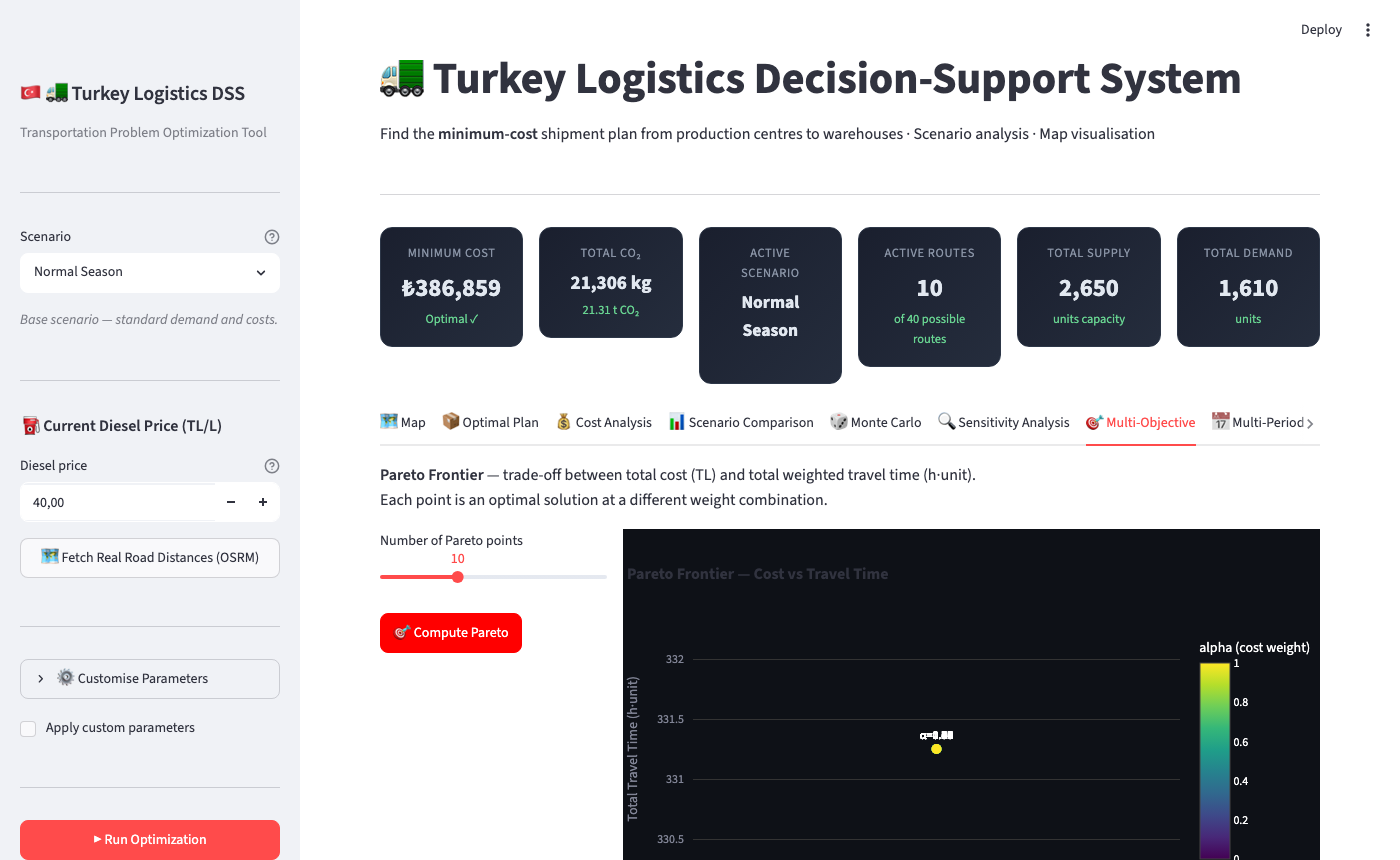
\includegraphics[width=\linewidth]{fig_pareto.png}
  \caption{Pareto frontier: total cost (TL) vs.\ total weighted travel
           time (h$\cdot$unit).}
  \label{fig:pareto}
\end{figure}

%=======================================================================
\section{Extensions}
\label{sec:extensions}

\subsection{Multi-Period Planning}

The four-quarter LP adds inventory variables $\text{inv}_{i,t} \geq 0$
and balance constraints:
$\text{inv}_{i,t} = \text{inv}_{i,t-1} + \text{prod}_i - \sum_j x_{ijt}$.
Seasonal demand multipliers per scenario shift quarterly load, and
holding costs $h$ penalise excess inventory.

\begin{figure}[htbp]
  \centering
  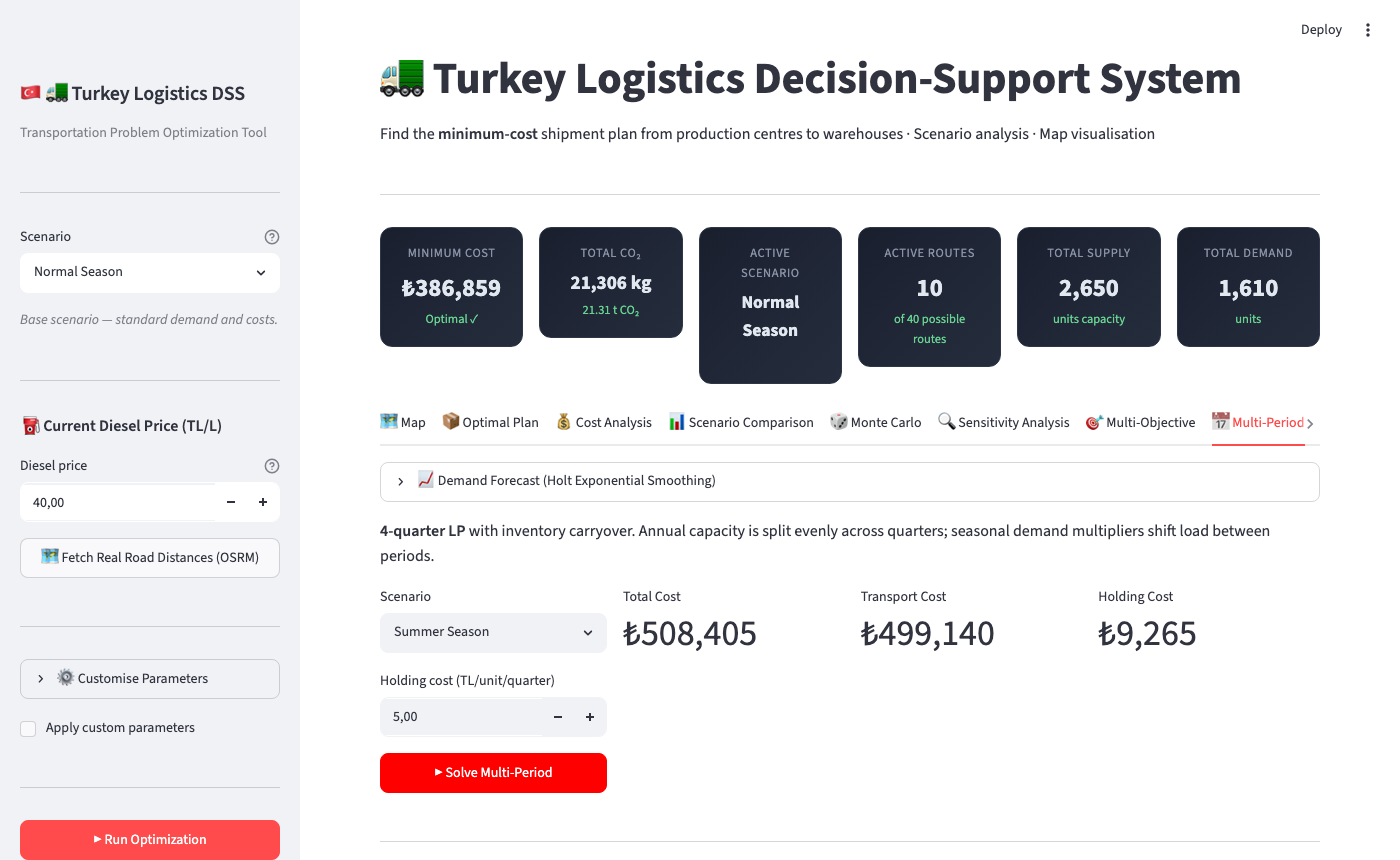
\includegraphics[width=\linewidth]{fig_multiperiod.png}
  \caption{Multi-period LP: stacked transport/holding costs per quarter
           and end-of-quarter inventory (right axis).}
  \label{fig:multiperiod}
\end{figure}

\subsection{Demand Forecasting}

Holt's double-exponential smoothing is applied to eight quarters of
synthetic historical demand generated with trend ($\times 0.93$--$1.07$),
seasonality ($\times [1.00, 1.10, 1.20, 0.90]$), and Gaussian noise.
Level $L_t$ and trend $T_t$ are updated as:
\begin{align*}
  L_t &= \alpha x_t + (1-\alpha)(L_{t-1} + T_{t-1}) \\
  T_t &= \beta(L_t - L_{t-1}) + (1-\beta)T_{t-1}
\end{align*}
with $h$-step forecasts $\hat{x}_{t+h} = L_t + h\,T_t$.
Default parameters $\alpha = 0.40$, $\beta = 0.15$ are user-adjustable.

\begin{figure}[htbp]
  \centering
  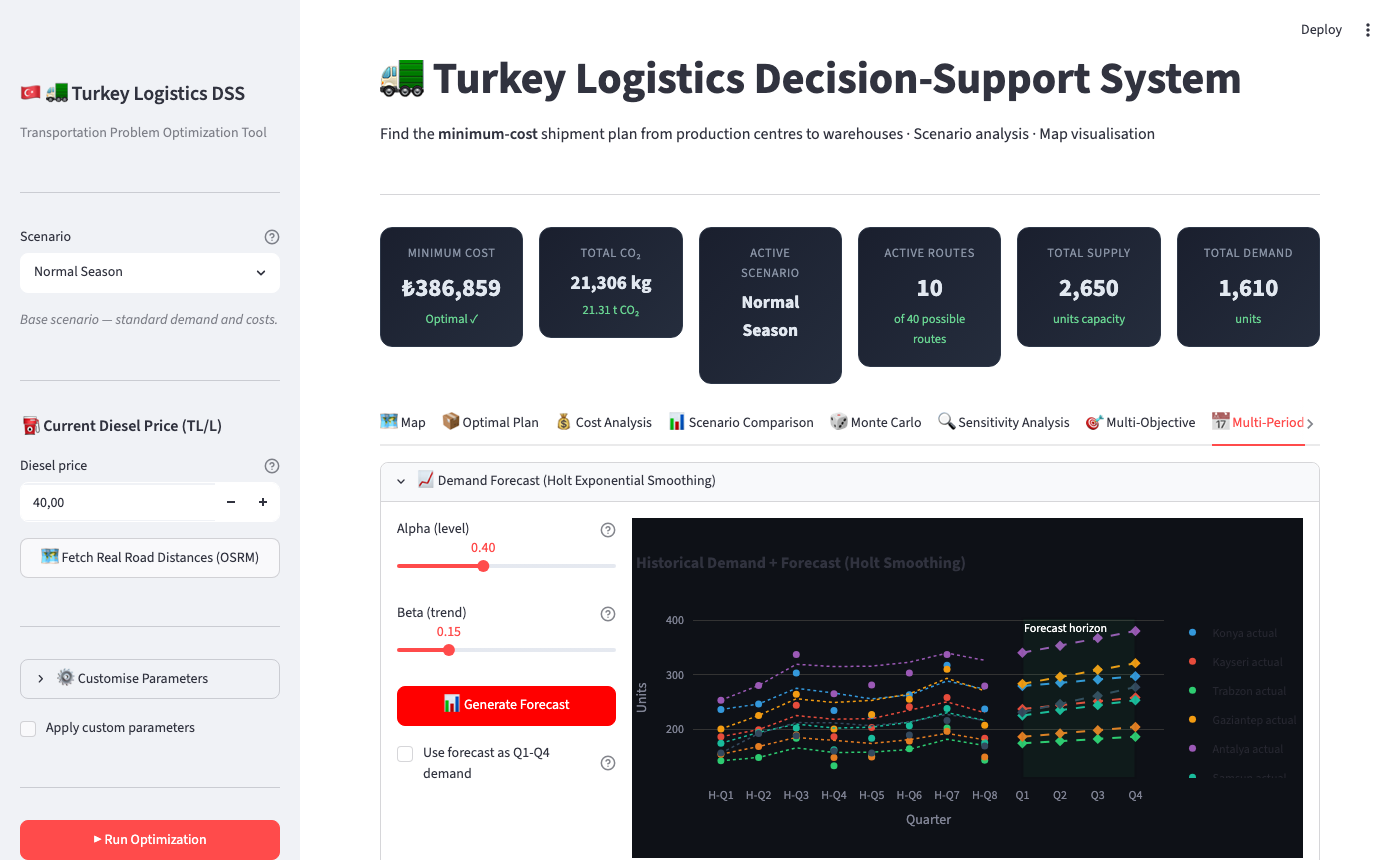
\includegraphics[width=\linewidth]{fig_forecast.png}
  \caption{Holt smoothing: historical demand (markers), fitted levels
           (dotted), and 4-quarter forecast (dashed) per warehouse.}
  \label{fig:forecast}
\end{figure}

\subsection{Disruption Simulation}

The disruption module sets selected source capacities to zero
(or scales them by a user-specified fraction $\rho \in (0,1)$)
and re-solves the LP.
The cost delta $\Delta Z = Z_\text{dis} - Z_\text{base}$ and the sets
of lost and new routes are reported, together with a colour-coded map
(blue = unchanged, red = lost, green = new routes).

\begin{figure}[htbp]
  \centering
  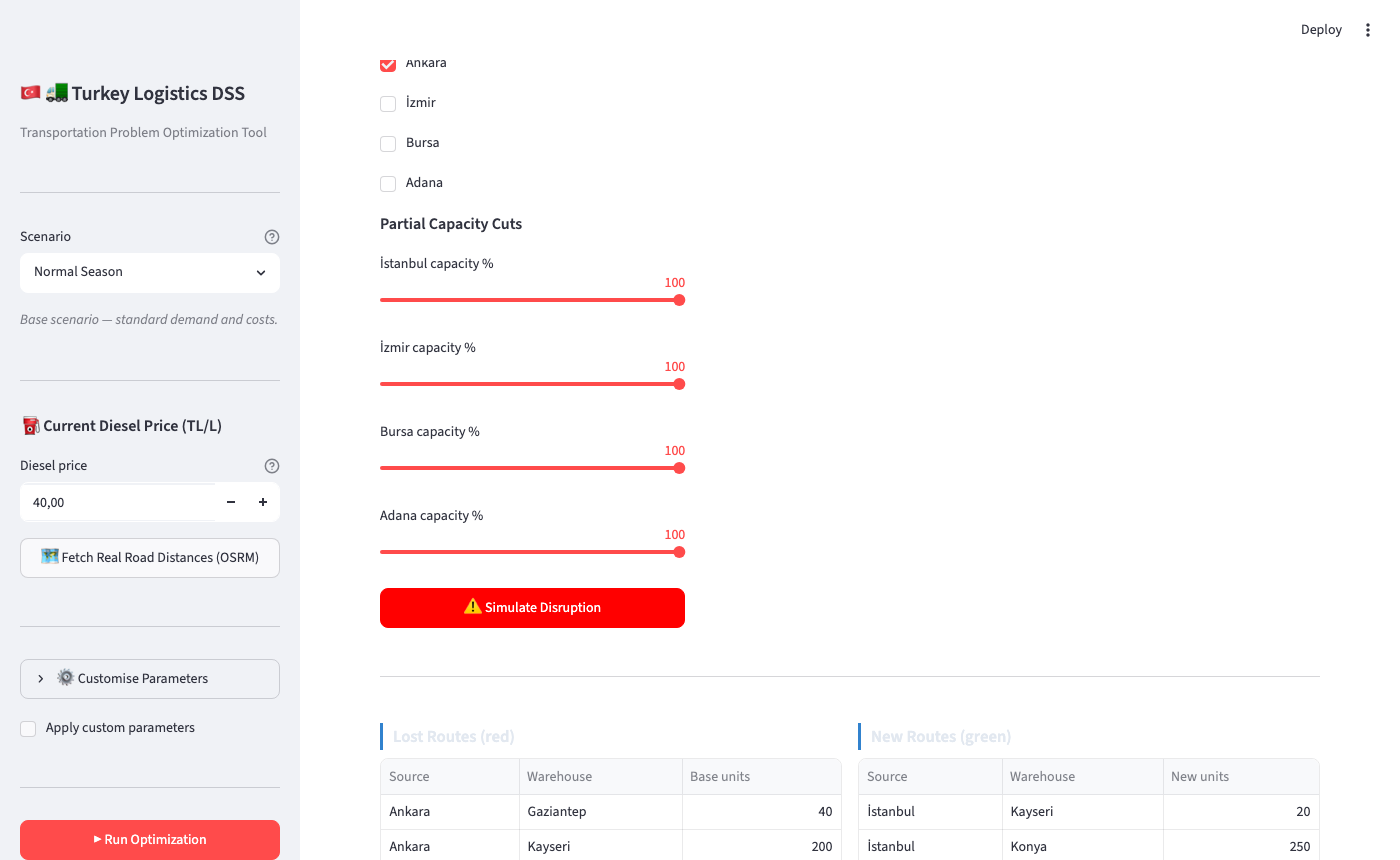
\includegraphics[width=\linewidth]{fig_disruption.png}
  \caption{Disruption simulation: cost delta metrics and colour-coded
           route map after disabling a production centre.}
  \label{fig:disruption}
\end{figure}

\subsection{P-Median Facility Location}

Given $M$ candidate city locations and demand weights $d_j$,
the p-median MIP selects $p$ facilities to minimise total
demand-weighted distance:

\begin{equation}
  \min\;\sum_{i \in J}\sum_{j \in C} d_i \cdot \delta_{ij} \cdot x_{ij}
\end{equation}
\begin{align*}
  \sum_{j} y_j &= p, \quad
  \sum_{j} x_{ij} = 1\;\forall i, \quad
  x_{ij} \leq y_j\;\forall i,j \\
  x_{ij},\, y_j &\in \{0,1\}
\end{align*}

where $C$ is the set of 13 candidate cities (5 sources + 8 warehouses),
$\delta_{ij}$ is the haversine distance, and $y_j = 1$ if facility $j$
is opened.
An elbow curve plots total weighted distance vs.\ $p$ to guide selection.

\begin{figure}[htbp]
  \centering
  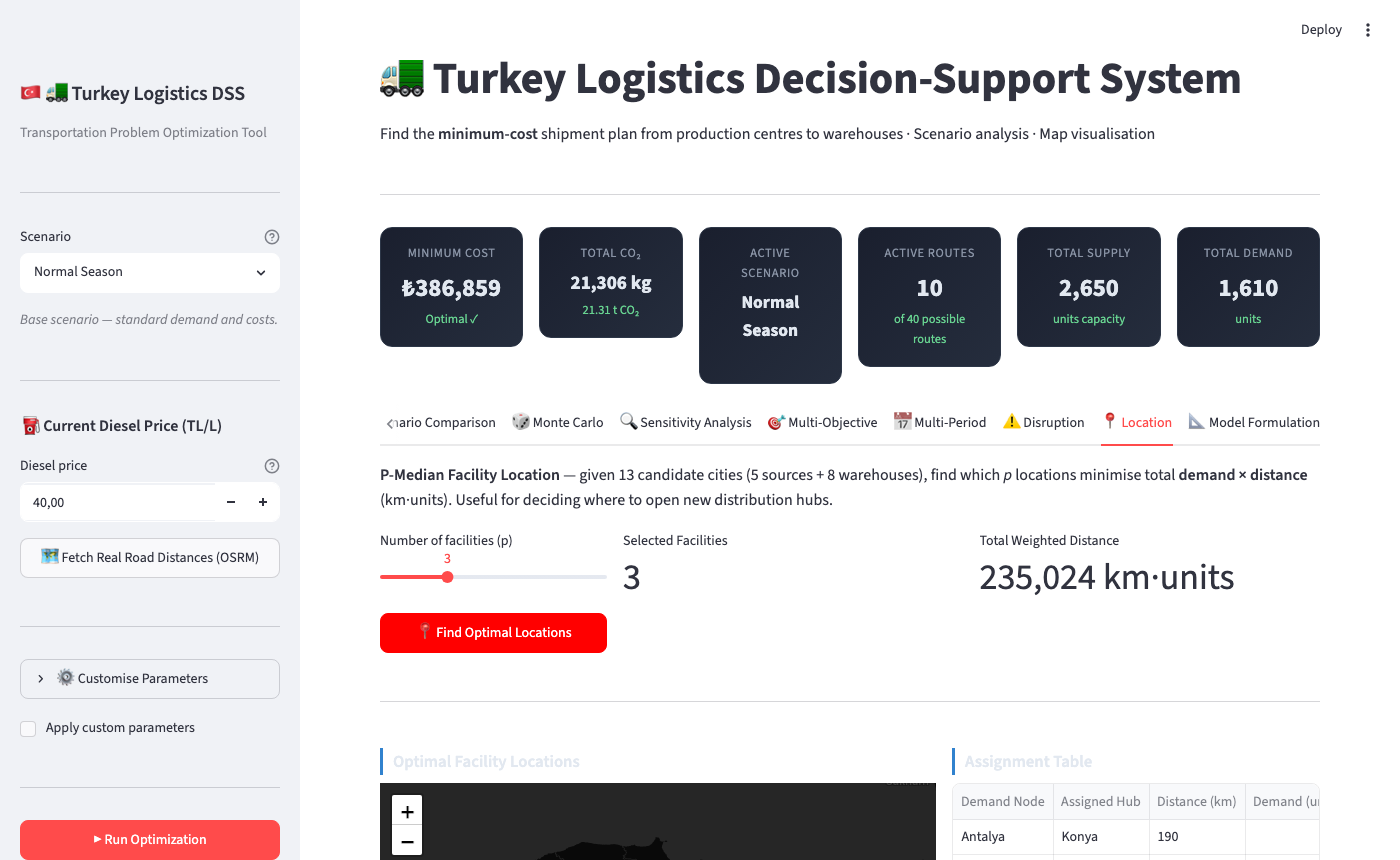
\includegraphics[width=\linewidth]{fig_location.png}
  \caption{P-Median result ($p = 3$): selected hubs (large coloured
           circles), demand node assignments (coloured lines), and
           elbow curve (inset).}
  \label{fig:location}
\end{figure}

%=======================================================================
\section{Conclusion}
\label{sec:conclusion}

This paper presented the Turkey Logistics DSS, an end-to-end transportation
optimisation platform combining classical LP with eight decision-support
extensions.
The system demonstrates:
\begin{enumerate}
  \item LP-based transportation models can be embedded in interactive
        web dashboards without sacrificing solver performance;
  \item shadow-price dashboards and scenario managers substantially
        reduce the cognitive overhead of what-if analysis;
  \item Monte Carlo simulation and Holt forecasting bridge the gap
        between deterministic optima and real-world demand variability;
  \item supply disruption simulation provides rapid re-routing insights
        without manual replanning;
  \item the p-median MIP offers a principled alternative to heuristic
        hub-selection methods;
  \item a REST API (FastAPI) and a pytest suite (124 tests) make the
        platform suitable for integration in larger supply-chain pipelines.
\end{enumerate}

%=======================================================================
\begin{thebibliography}{9}

\bibitem{hillier}
F.~S. Hillier and G.~J. Lieberman,
\textit{Introduction to Operations Research}, 11th~ed.
McGraw-Hill, 2021.

\bibitem{winston}
W.~L. Winston,
\textit{Operations Research: Applications and Algorithms}, 4th~ed.
Cengage Learning, 2004.

\bibitem{pulp}
S.~Mitchell, M.~O'Sullivan, and I.~Dunning,
``PuLP: A Linear Programming Toolkit for Python,''
\textit{University of Auckland}, 2011.
[Online]. Available: \url{https://github.com/coin-or/pulp}

\bibitem{cbc}
J.~Forrest \textit{et al.},
``CBC: COIN-OR Branch and Cut,''
COIN-OR Foundation, 2005--2024.
[Online]. Available: \url{https://github.com/coin-or/Cbc}

\bibitem{streamlit}
Streamlit Inc.,
``Streamlit: The fastest way to build and share data apps,''
2024. [Online]. Available: \url{https://streamlit.io}

\bibitem{osrm}
D.~Luxen and C.~Vetter,
``Real-time routing with OpenStreetMap data,''
in \textit{Proc. 19th ACM SIGSPATIAL}, Chicago, IL, 2011, pp.~513--516.

\bibitem{folium}
R.~Story,
``Folium: Python Data, Leaflet.js Maps,''
2013--2024. [Online]. Available: \url{https://github.com/python-visualization/folium}

\bibitem{plotly}
Plotly Technologies Inc.,
``Collaborative data science,''
Montr\'{e}al, QC, 2015. [Online]. Available: \url{https://plotly.com}

\bibitem{docker}
Docker Inc.,
``Docker: Accelerated Container Application Development,''
2024. [Online]. Available: \url{https://www.docker.com}

\bibitem{ipcc}
IPCC,
``2006 IPCC Guidelines for National Greenhouse Gas Inventories,
Volume 2: Energy,'' IGES, Japan, 2006.

\bibitem{holt}
C.~C. Holt,
``Forecasting seasonals and trends by exponentially weighted moving averages,''
\textit{Int. J. Forecast.}, vol.~20, no.~1, pp.~5--10, 2004.

\bibitem{hakimi}
S.~L. Hakimi,
``Optimum locations of switching centers and the absolute centers and medians
of a graph,''
\textit{Oper. Res.}, vol.~12, no.~3, pp.~450--459, 1964.

\end{thebibliography}

\end{document}
